\begin{document}
The circuits required only minor changes from simulation to experimental implementation.	
	

\subsection{NMOS amplifier}
The final circuit is shown in Figure \ref{fig:finalexperimentalschem}.
\begin{figure}[H]
	\centering
	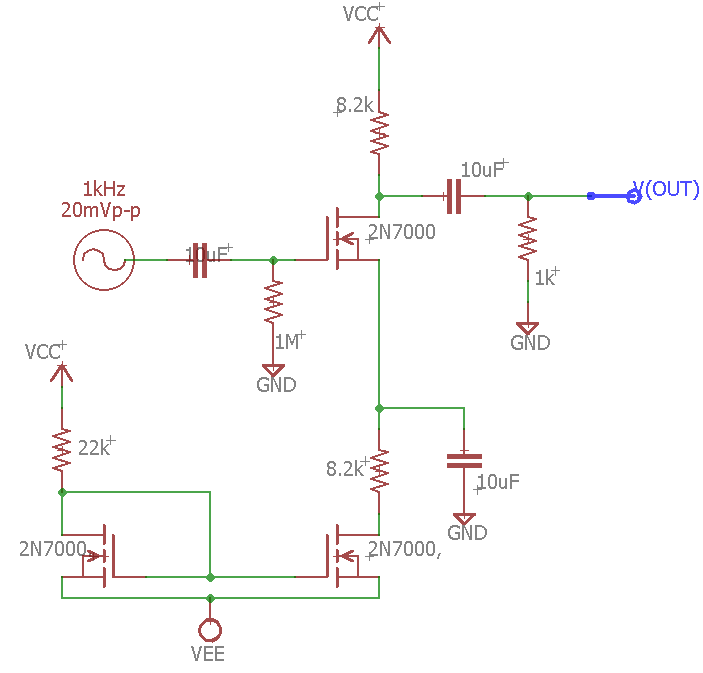
\includegraphics[width=0.7\linewidth]{ExperimentalImplementation/NMOS_exp}
	\caption{NMOS final circuit schematic}
	\label{fig:nmosexp}
\end{figure}



\begin{figure}[H]
	\centering
	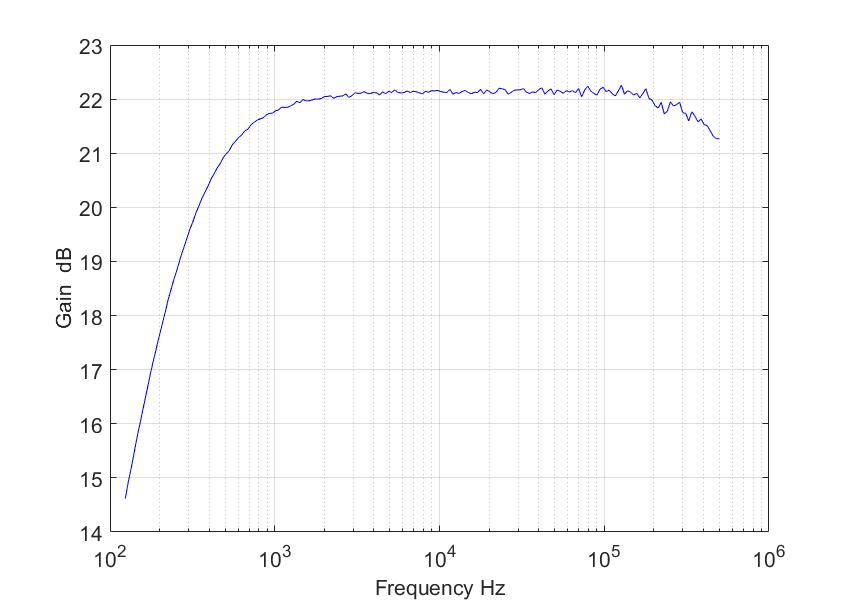
\includegraphics[width=0.7\linewidth]{ExperimentalImplementation/nmosamp.jpg}
	\caption{NMOS experimental frequency response}
	\label{fig:nmosfreq}
\end{figure}

\begin{figure}[H]
	\centering
	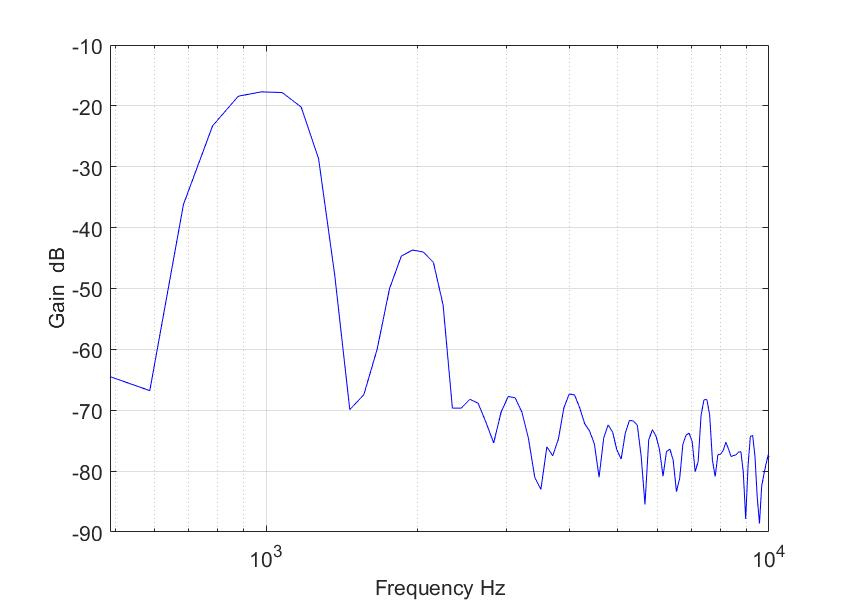
\includegraphics[width=0.7\linewidth]{ExperimentalImplementation/nmos_fft.jpg}
	\caption{NMOS experimental FFT}
	\label{fig:nmosfft}
\end{figure}




\begin{table}[H]
	\centering
	\caption{NMOS experimental values}
	\label{tab:nmosexp}
	\begin{tabular}{cc}
		$Q_1, Q_2, Q_3$ & 2N7000        \\ \hline
		$R_ref$         & 22 k$\Omega$ \\ \hline
		$R_g$           & 1 M$\Omega$  \\ \hline
		$R_d$           & 8.2 k$\Omega$   \\ \hline
		$R_s$           & 8.2 k$\Omega$  \\ \hline
		$R_L$           & 1k$\Omega$    \\ \hline
		$C_B, C_C, C_E$ & 10 $\mu$F         \\ \hline   
	\end{tabular}
\end{table}



\subsection{BJT amplifier}


\begin{figure}[H]
	\centering
	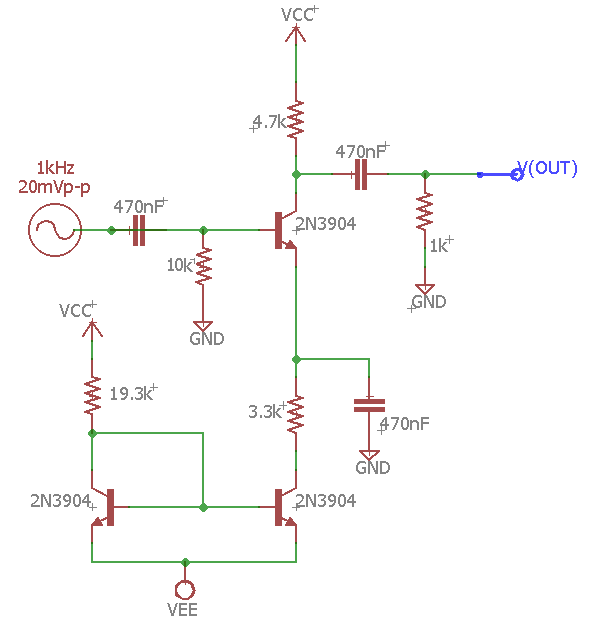
\includegraphics[width=0.7\linewidth]{ExperimentalImplementation/BJT_Exp}
	\caption{BJT final schematic}
	\label{fig:bjtexp}
\end{figure}



\begin{figure}[H]
	\centering
	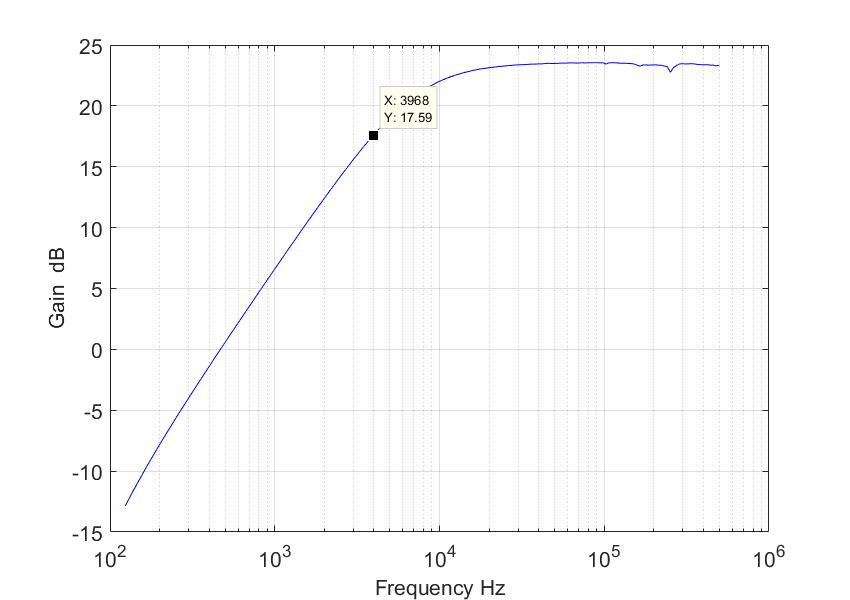
\includegraphics[width=0.7\linewidth]{ExperimentalImplementation/bjt_outputexp.jpg}
	\caption{BJT experimental frequency response}
	\label{fig:bjtexpfreq}
\end{figure}


\begin{figure}[H]
	\centering
	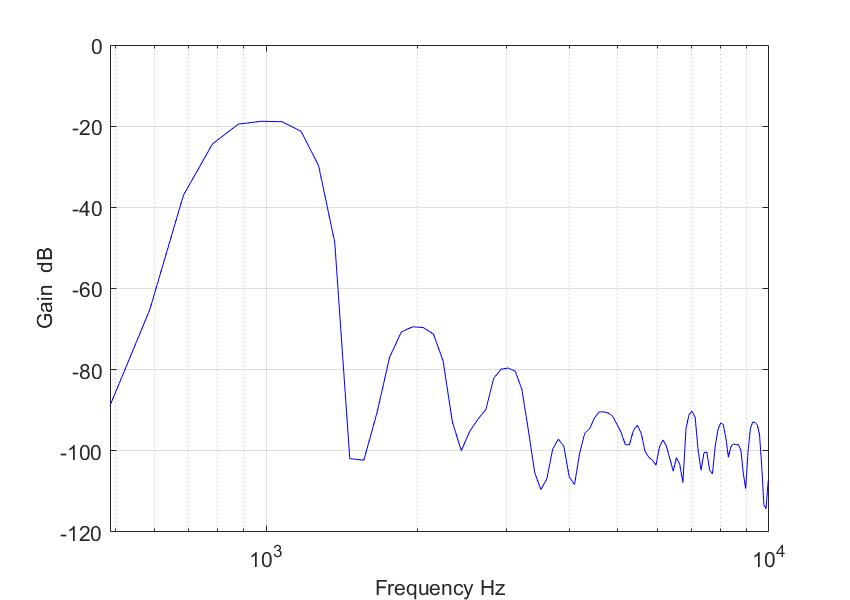
\includegraphics[width=0.7\linewidth]{ExperimentalImplementation/bjt_fft.jpg}
	\caption{BJT experimental FFT}
	\label{fig:bjtexpfft}
\end{figure}




\begin{table}[H]
	\centering
	\caption{BJT experimental values}
	\label{tab:bjtexp}
	\begin{tabular}{cc}
		$Q_1, Q_2, Q_3$ & 2N3904        \\ \hline
		$R_ref$         & 19.3k$\Omega$ \\ \hline
		$R_C$           & 4.7k$\Omega$  \\ \hline
		$R_B$           & 10k$\Omega$   \\ \hline 
		$R_E$           & 3.3k$\Omega$  \\ \hline 
		$R_L$           & 1k$\Omega$    \\ \hline
		$C_B, C_C, C_E$ & 470nF        \hline
	\end{tabular}
\end{table}

In order to meet specifications, several minor changes to all circuits were made. The individual changes are discussed in their respective subsection as follows, the signal conditioner then the current driver.


%\subsection{Ring oscillator}
%\subfile{ExperimentalImplementation/ringosc.tex}



\end{document}